\documentclass[10pt,twocolumn,letterpaper]{article}

\usepackage{cvpr}
\usepackage{times}
\usepackage{epsfig}
\usepackage{graphicx,caption}
% * <yl2363@cornell.edu> 2016-12-13T04:05:19.045Z:
%
% ^.
\usepackage{amsmath}
\usepackage{amssymb}
\usepackage[shortlabels]{enumitem}
\usepackage{threeparttable}

\usepackage{url}
\usepackage[english]{babel}
\usepackage{amsfonts}
\usepackage{subfigure}

\newcommand{\yixuan}{\textcolor{blue}}
\newcommand{\todo}{\textcolor{red}}
\newcommand{\vpara}[1]{\vspace{0.1in}\noindent\textbf{#1}}


% Include other packages here, before hyperref.

% If you comment hyperref and  then uncomment it, you should delete
% egpaper.aux before re-running latex.  (Or just hit 'q' on the first latex
% run, let it finish, and you should be clear).
\usepackage[pagebackref=true,breaklinks=true,letterpaper=true,colorlinks,bookmarks=false]{hyperref}

\cvprfinalcopy % *** Uncomment this line for the final submission

\def\cvprPaperID{2100} % *** Enter the CVPR Paper ID here
\def\httilde{\mbox{\tt\raisebox{-.5ex}{\symbol{126}}}}

% Pages are numbered in submission mode, and unnumbered in camera-ready
 \ifcvprfinal\pagestyle{empty}\fi
\begin{document}

%%%%%%%%% TITLE
\title{Stacked Generative Adversarial Networks}

% \author{Xun Huang \\
% \author{Authors \\
% Cornell University\\
% Alpha University\\
% Institution1 address\\
% {\tt\small xh258@cornell.edu}
% {\tt\small secondauthor@i2.org}
% For a paper whose authors are all at the same institution,
% omit the following lines up until the closing ``}''.
% Additional authors and addresses can be added with ``\and'',
% just like the second author.
% To save space, use either the email address or home page, not both
% Second Author\\
% Institution2\\
% First line of institution2 address\\
% {\tt\small secondauthor@i2.org}
% }

\author{Xun Huang$^{1}$ \qquad Yixuan Li$^{2}$ \qquad Omid Poursaeed$^{2}$  \qquad John Hopcroft$^{1}$ \qquad Serge Belongie$^{1,3}$ \\
	$^1${Department of Computer Science, Cornell University}\\
    $^2${School of Electrical and Computer Engineering, Cornell University}\quad
	$^3${Cornell Tech}\\
	{\tt\small \{xh258,yl2363,op63,sjb344\}@cornell.edu jeh@cs.cornell.edu}
}



\maketitle
%\thispagestyle{empty}

%%%%%%%%% ABSTRACT
\begin{abstract}
% Deep neural networks (DNNs) have become a dominant approach in a wide range of machine learning tasks. While most of the success has been enjoyed by bottom-up networks trained for discriminative tasks (\emph{e.g.}, convolutional neural networks (CNNs)), learning top-down deep generative models has started to attract increasing attention.  However, the strength of current state-of-the-art deep generative models still significantly lag behind their discriminative counterparts. 
In this paper, we propose a novel generative model named Stacked Generative Adversarial Networks (SGAN), which is trained to invert the hierarchical representations of a bottom-up discriminative network. Our model consists of a top-down stack of GANs, each learned to generate lower-level representations conditioned on higher-level representations. A representation discriminator is introduced at each feature hierarchy to encourage the representation manifold of the generator to align with that of the bottom-up discriminative network, leveraging the powerful discriminative representations to guide the generative model. In addition, we introduce a conditional loss that encourages the use of conditional information from the layer above, and a novel entropy loss that maximizes a variational lower bound on the conditional entropy of generator outputs. We first train each stack independently, and then train the whole model end-to-end. Unlike the original GAN that uses a single noise vector to represent all the variations, our SGAN decomposes variations into multiple levels and gradually resolves uncertainties in the top-down generative process. Based on visual inspection, Inception scores and visual Turing test, we demonstrate that SGAN is able to generate images of much higher quality  than GANs without stacking. 
\end{abstract}

%%%%%%%%% BODY TEXT
\vspace{-0.15in}
\section{Introduction}
\label{intro}

Recent years have witnessed tremendous success of deep neural networks~(DNNs), especially the kind of bottom-up neural networks trained for discriminative tasks. In particular, Convolutional Neural Networks (CNNs) have achieved  impressive accuracy on the challenging ImageNet classification benchmark \cite{krizhevsky2012imagenet,simonyan2015very,szegedy2015going,he2016deep,russakovsky2015imagenet}. Interestingly, it has been shown that CNNs trained on ImageNet for classification can learn representations that are transferable to other tasks \cite{sharif2014cnn}, and even to other modalities \cite{gupta2016cross}.  However, bottom-up discriminative models are focused on learning useful representations from data, being incapable of capturing the data distribution. 


Learning top-down generative models that can explain complex data distribution is a long-standing problem in machine learning research. The expressive power of deep neural networks makes them natural candidates for generative models, and several recent works have shown promising results \cite{kingma2014auto, goodfellow2014generative, oord2016pixel, li2015generative, zhao2016energy,makhzani2016adversarial,dosovitskiy2015learning}. 
% However, the current state-of-the-art deep generative models still significantly lag behind their discriminative counterparts. 
While state-of-the-art DNNs can rival human performance in certain discriminative tasks, current best deep generative models still fail when there are large variations in the data distribution. 

A natural question therefore arises: can we leverage
the hierarchical representations in a 
%bottom-up and 
discriminatively trained model to help the learning of top-down generative models? In this paper, we propose a generative model named {\em Stacked Generative Adversarial Networks} (SGAN). %, which effectively leverages the rich bottom-up deep representations when training a generative model. 
Our model consists of a top-down stack of GANs, each trained to generate ``plausible'' lower-level representations conditioned on higher-level representations. Similar to the image discriminator in the original GAN model which is trained to distinguish ``fake'' images from ``real'' ones, we introduce a set of \emph{representation discriminators} that are trained to distinguish ``fake'' representations from ``real'' representations. The \emph{adversarial loss} introduced by the representation discriminator forces the intermediate representations of the SGAN to lie on the manifold of the bottom-up DNN's representation space. %, providing guidance from the powerful discriminative models. 
In addition to the adversarial loss, we also introduce a \emph{conditional loss} that imposes each generator to use the higher-level conditional information, and a novel \emph{entropy loss} that  encourages each generator to generate diverse representations. 
By stacking several GANs in a top-down way and using the top-most GAN to receive labels and the bottom-most GAN to generate images, SGAN can be trained to model the data distribution conditioned on class labels. 
%In a series of experiments, we demonstrate the effectiveness of our SGAN. 
Through extensive experiments, we demonstrate that our SGAN is able to generate images of much higher quality than a vanilla GAN. In particular, our model obtains state-of-the-art Inception scores on CIFAR-10 dataset.
%, SGAN has three substantial advantages: 
%\begin{enumerate}
%\item {\bf Quality}. SGAN decomposes the difficult image generation task into several easier sub-tasks by leveraging the discriminative representations. As a result, SGAN can generate higher-quality samples than a vanilla GAN. 
%%Empirically, we also observe SGAN to be more stable than a vanilla GAN.
%\item {\bf Diversity}. With the proposed entropy loss, SGAN can avoid the (conditional) \emph{model collapse} phenomenon that is common in (conditional) GAN training, thus being able to generate more diverse samples.
%\item {\bf Interpretability}. Our SGAN is more interpretable than a vanilla GAN in that it uses different levels of noise variables to represent different levels of variations.
%\end{enumerate}

%is (1) more powerful, because it decomposes image generation into several easier steps by leveraging the discriminative representations (2) more diverse samples, entropy loss (3) more interpretable, decompose
%Our method offers several advanes compared to a vanilla GAN:
%\begin{enumerate}
%\item transfermultiple-level factors of variations learning
%\item 
%\end{enumerate}
%
%In the remainder of the paper, 
%manifold on the representation space
%
%perfect disentangling -> density is flat 
%higher-level manifold -> most configurations are likely, locally uniform distribution

\section{Related Work}
\label{related}
\vspace{-0.1in}
\vpara{Deep Generative Image Models.}
There has been a large body of work on generative image modeling with deep learning. Some early efforts include Restricted Boltzmann Machines \cite{hinton2002training} and Deep Belief Networks \cite{hinton2006reducing}.
More recently, several successful paradigms of deep generative models have emerged, including the auto-regressive models \cite{larochelle2011neural,germain2015made,theis2015generative,oord2016pixel,oord2016conditional,gregor2014deep}, Variational Auto-encoders (VAEs) \cite{kingma2014auto,kingma2014semi,rezende2014stochastic,yan2016attribute2image,gregor2015draw}, and Generative Adversarial Networks (GANs) \cite{goodfellow2014generative, denton2015deep, radford2016unsupervised, reed2016generative,salimans2016improved,larsen2016autoencoding}. Our work builds upon the GAN framework, which employs a generator that transforms a noise vector into an image and a discriminator that distinguishes between real and generated images.
%The generator is trained to generate images that are real enough to ``fool'' the discriminator.
%In particular, our work is reminiscent of  the Deep Belief Networks (DBN) \cite{hinton2006reducing} in that both models are top-down generative models composed of several hierarchies, each representing the distribution of lower-level representations conditioned on higher-level representations. However, DBN is usually trained by learning a bottom-up stack of RBMs, while our model consists of a top-down stack of GANs.
%One of the important differences is that all our hidden neurons are deterministic while 
%A wide variety of deep learning approaches involve generative parametric models. Restricted Boltzmann machines [13, 16, 19, 21], Deep Boltzmann machines [24, 7], Denoising auto-encoders [28] all have a generative decoder that reconstructs the image from the latent representation. Variational auto-encoders [15, 22] provide probabilistic interpretation which facilitates sampling. However, for all these methods convincing samples have only been shown on simple datasets such as MNIST and NORB, possibly due to training complexities which limit their applicability to larger and more realistic images.
%Several

%More recently, several successful paradigms of deep generative models have emerged. Auto-regressive models \cite{larochelle2011neural,germain2015made,theis2015generative,oord2016pixel,oord2016conditional} decompose the image joint distribution into a product of conditional distributions over all pixels and generate the image in a pixel-by-pixel manner. Variational Auto-encoders (VAEs) \cite{kingma2013auto,kingma2014semi,rezende2014stochastic} adopt an auto-encoder architecture with a stochastic bottle-neck layer, trained to maximize a variational lower bound on the data likelihood. Our work builds upon the recent Generative adversarial networks (GANs) \cite{goodfellow2014generative, denton2015deep, radford2015unsupervised} framework, which uses a generator to transform a noise vector into an image. The generator is trained to generate images that are real enough to ``fool'' a discriminator.


%Recently, Generative Adversarial Networks (GANs) \cite{goodfellow2014generative} have emerged as a powerful framework to generate images of high visual fidelity. both trained to \cite{radford2015unsupervised} further introduces a deep convolutional version of GANs. \cite{mirza2014conditional, gauthier2014conditional} propose a conditional version of GAN by feeding the conditional information to both the generator and discriminator. However, GANs are known to be very difficult to train. \cite{salimans2016improved} introduce several heuristic techniques that encourage training convergence. 

However, due to the vast variations in image content, it is still challenging for GANs to generate diverse images with sufficient details. %When there are vast variations in the image content, \emph{i.e.}, the entropy $H(P_{data}(x))$ is high, the generator either completely fail or significantly underestimate the entropy of the data distribution. 
To this end, several works have attempted to factorize a GAN into a series of GANs, decomposing the difficult task into several more tractable sub-tasks. Denton~\etal~\cite{denton2015deep} propose a LAPGAN model that factorizes the generative process  into multi-resolution GANs, with each GAN generating a higher-resolution residual conditioned on a lower-resolution image. Although both LAPGAN and SGAN consist of a sequence of GANs each working at one scale, LAPGAN focuses on generating \emph{multi-resolution images} from coarse to fine while our SGAN aims at modeling \emph{multi-level representations} from abstract to specific. %\cite{kwak2016generating} use multiple GANs to generate different parts of the image and finally combine these parts with alpha-blinding.
Wang and Gupta~\cite{wang2016generative} propose a $\mathrm{S^{2}}$-GAN, using one GAN to generate  surface normals and another GAN to generate images conditioned on surface normals. Surface normals can be viewed as a specific type of image representations, capturing the underlying 3D structure of an indoor scene. On the other hand, our framework can leverage the more general and powerful multi-level representations in a pre-trained discriminative DNN. 

There are several works that use a pre-trained discriminative model to aid the training of a generator. \cite{lamb2016discriminative, dosovitskiy2016generating} add a regularization term that encourages the reconstructed image to be similar to the original image in the feature space of a discriminative network. \cite{ulyanov2016texture,johnson2016perceptual} use an additional ``style loss'' based on Gram matrices of feature activations. Different from our method, all the works above only add loss terms to regularize the generator's \emph{output}, without regularizing its \emph{internal representations}. 
%Our SGAN adopts a very different approach, using adversarial training to encourage the internal representations of the generator to reside on the representation manifold defined by a pre-trained discriminative model.  

\vpara{Matching Intermediate Representations Between Two DNNs.} There have been some works that attempt to ``match'' the intermediate representations between two DNNs. \cite{romero2015fitnets, gupta2016cross} use the intermediate representations of one pre-trained DNN to guide another DNN in the context of knowledge transfer. 
%For example, in \cite{romero2014fitnets, gupta2015cross} the representations in a guided layer of a ``student network'' is used to regress the representations in a hint layer of a ``teacher network'', and the regression error is back-propagated to the student network. 
%\cite{gupta2015cross} adopt a similar paradigm but use a teacher network trained on ImageNet to guide a student network trained with depth images. 
Our method can be considered as a special kind of knowledge transfer. However, we aim at transferring the knowledge in a bottom-up DNN  to a top-down generative model, instead of another bottom-up DNN. 
Also, some auto-encoder architectures employ layer-wise reconstruction loss~\cite{valpola2015neural,rasmus2015semi,zhao2016stacked,2016-icml-recon-dec}. % include reconstruction loss at every layer of the decoder to encourage the intermediate representations of the decoder to be similar to those of the encoder. 
The layer-wise loss is usually accompanied by lateral connections from the encoder to the decodery. On the other hand, SGAN is a generative model and does not require any information from the encoder once training completes. Another important difference % of our approach from the two lines of work above 
is that we use adversarial loss instead of $L2$ reconstruction loss to match intermediate representations. 

%Also, note that an important difference of our approach from the two lines of work is the adversarial training strategy we used: we do not enforce the intermediate representations of the generator to be the same as any particular intermediate representations in the training set. Instead, they are only required to reside on the manifold of the representation space. 
%These architectures relieve the burden of higher layers to represent every details and enable the higher layers to focus on learning invariant representations.  

%Our method is different from the two lines of work in two important aspects. First, we are aiming at learning a purely top-down generative model. Unlike \cite{romero2014fitnets,gupta2015cross} that transfer the knowledge in a bottom-up encoder to another bottom-up encoder, we transfer the knowledge to a top-down generator. Also, the decoder in \cite{rasmus2015semi,zhao2015stacked} can only do reconstruction while our generator is capable of capturing the data distribution. Another difference is the adversarial training strategy we used. We do not enforce the intermediate representations of our generator to be the same as any particular intermediate representations in the training set. Instead, they are only required to reside on the manifold in the representation space. 
%One discriminator at each level of the representation hierarchy is introduced to distinguish the intermediate representations of the generator from the intermediate representations produced by an encoder. 

\vpara{Visualizing Deep Representations.}
Our work is also related to the recent efforts in visualizing the internal representations of DNNs. One popular approach uses gradient-based optimization to find an image whose representation is close to the one we want to visualize \cite{mahendran2016visualizing}. 
%\cite{ dai2014generative, mahendran2015understanding, mahendran2016visualizing,nguyen2016multifaceted}. 
%Usually, a handcrafted natural image prior is employed  to preserve the naturalness of the image. % gradient descent v.s. train a deconvnet
%One popular approach to invert representations to image space is to apply gradient-based optimization on the inputs to find an image whose representation is close to the representation code we want to visualize 
%More related to our method is another approach of training a deconvolutional network that transforms an intermediate feature representation to an image via one top-down pass.  %\cite{zeiler2014visualizing} use a deconvolutional network with the same architecture as the convolutional network to be visualized, but in a reverse direction. The filters in each deconvolutional layer are fixed to the transposed filters in the corresponding convolutional layer, and switch variables in the pooling layers are passed to the un-pooling layers in the deconvolutional network. 
Other approaches, such as \cite{dosovitskiy2016inverting}, train a top-down deconvolutional network to reconstruct the input image from a feature representation by minimizing the Euclidean reconstruction error in image space. However, there is inherent uncertainty in the reconstruction process, since the representations in higher layers of the DNN are trained to be invariant to irrelevant transformations and to ignore low-level details. With Euclidean training objective, the deconvolutional network tends to produce blurry images. 
To alleviate this problem, Dosovitskiy abd Brox~\cite{dosovitskiy2016generating} further propose a feature loss and an adversarial loss that enables much sharper reconstructions.  
% \cite{nguyen2016synthesizing} use a pre-trained, fixed deconvolutional network in \cite{dosovitskiy2016generating} to generate images that can maximize certain neuron activations in another bottom-up DNN. 
However, it still does not tackle the problem of uncertainty in reconstruction. Given a high-level feature representation, the deconvolutional network deterministically generates a single image, despite the fact that there exist many images having the same representation. Also, there is no obvious way to sample images because the feature prior distribution is unknown. Concurrent to our work, Nguyen~\etal~\cite{nguyen2016plug} incorporate the feature prior with a variant of denoising auto-encoder (DAE). Their sampling relies on an iterative optimization procedure, while we are focused on efficient feed-forward sampling.
%On the contrary, our SGAN is a fully-fledged generative model, capable of  capturing the data distribution $P_{data}(x)$ and sampling diverse images accordingly. 

\section{Methods}
\label{methods}

In this section we introduce our model architecture. In Sec.~\ref{GAN} we briefly overview the framework of Generative Adversarial Networks. We then describe our proposal for Stacked Generative Adversarial Networks in Sec.~\ref{SGAN}. In Sect.~\ref{Condloss} and \ref{Entloss} we will focus on our two novel loss functions, conditional loss and entropy loss, respectively. %Fig \ref{fig:sgan} shows an \textbf{overview of} our model architecture. 

\begin{figure*}[!htbp]
\centering
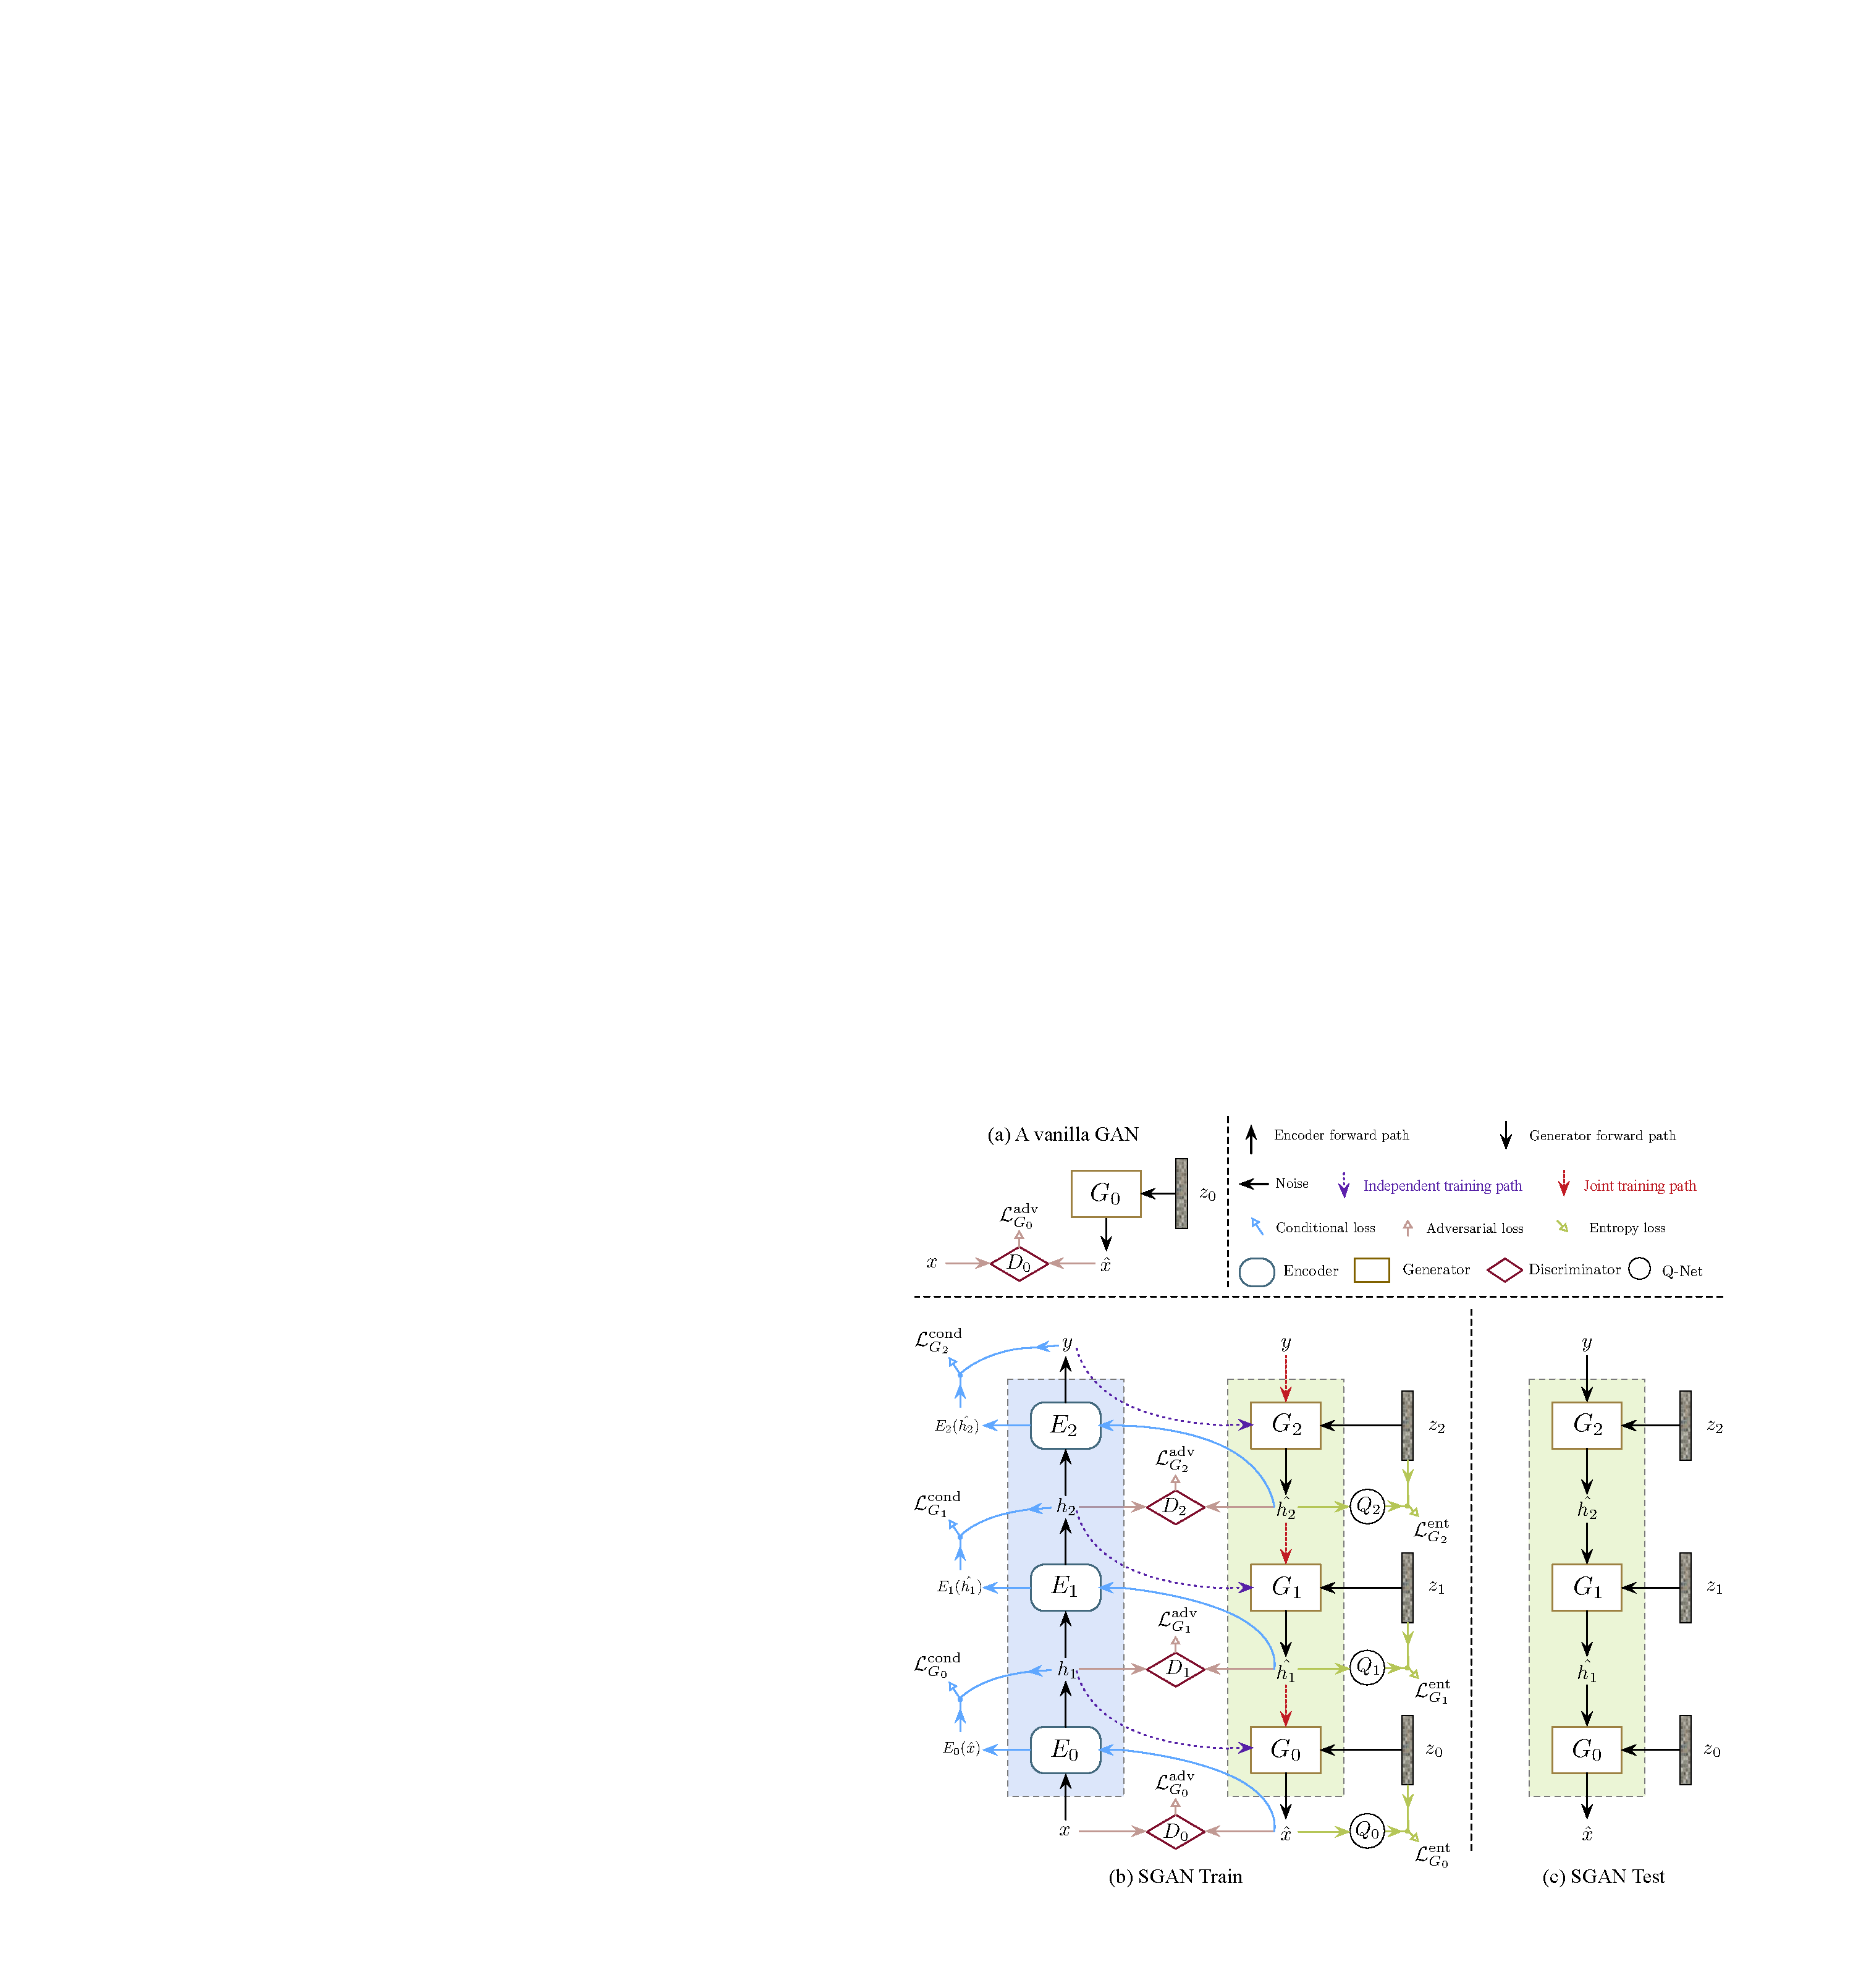
\includegraphics[width=0.9\linewidth]{figures/sgan-yixuan.pdf}
   \caption{\textbf{An overview of SGAN.} (a) The original GAN in~\cite{goodfellow2014generative}. (b) The workflow of training SGAN, where each generator $G_i$ tries to generate plausible features that can fool the corresponding representation discriminator $D_i$. Each generator receives conditional input from encoders in the independent training stage, and from the upper generators in the joint training stage. (c) New images can be sampled from SGAN (during test time) by feeding random noise to each generator $G_i$.}
\label{fig:sgan}
\vspace{-0.3cm}
\end{figure*}


\subsection{Background: Generative Adversarial Network}
\label{GAN}
As shown in Fig.~\ref{fig:sgan}~(a), the original GAN \cite{goodfellow2014generative} is trained using a two-player min-max game: a discriminator $D$ trained to distinguish generated images from real images, and a generator $G$ trained to fool $D$. The discriminator loss $\mathcal{L}_{D}$ and the generator loss $\mathcal{L}_{G}$ are defined as follows: 
\begin{equation}
\mathcal{L}_{D} =  \mathbb{E}_{x\sim P_{data}}[-\log D(x)] +\mathbb{E}_{z\sim P_{z}}[-\log (1-D\big(G(z))\big)] 
\end{equation} 
\begin{equation}
\mathcal{L}_{G} = \mathbb{E}_{z\sim P_{z}}[ -\log (D\big(G(z))\big)] 
\end{equation}

In practice, $D$ and $G$ are usually updated alternately. The training process matches the generated image distribution $P_{G}(x)$ with the real image distribution $P_{data}(x)$ in the training set. In other words, The adversarial training forces $G$ to generate images that reside on the natural images manifold. 

%In the original GAN framework, the single noise vector $z$ has to encapsulate every detail about an image. As a result, $z$ cannot focus on representing high-level invariant features because invariant features are by definition not sufficient to generate an image with enough details. 
% $z$ is also not very efficient at representing low-level spatial details because it does not have any spatial dimensions. 
%$A similar problem in the auto-encoders  has been discussed by ~\cite{valpola2015neural, rasmus2015semi, zhao2015stacked} and we refer readers to these papers for their solutions in the context of auto-encoders. 
%Intuitively, the total variations of images could be decomposed into multiple levels, with higher-level semantic variations (\emph{e.g.}, attributes, object categories, rough shapes) and lower-level spatial variations (\emph{e.g.}, detailed contours and textures, background clutters). A better approach would be to use different levels of noise variables to represent different levels of variations.
%Although \cite{salimans2016improved, zhao2016energy} have tried to feed multi-scale noise into different layers of the generator, there is nothing to teach their models to use noise variables at different levels to represent different levels of variations. %In the next section we will discuss how our SGAN could tackle this problem. % (NOTE)
% in GAN by decomposing the total variations of the image into different hierarchies, each represented by one noise variable. 




\subsection{Stacked Generative Adversarial Networks}
\label{SGAN}
%Fig \ref{fig:sgan} shows an overview of SGAN model architecture. 

\vpara{Pre-trained Encoder.} We first consider a bottom-up DNN pre-trained for classification, 
which is referred to as the encoder $E$ throughout. %$E$ is trained to learn powerful hierarchical representations that are not only helpful for classification but also transferable to other tasks. 
We define a stack of bottom-up deterministic nonlinear mappings: $h_{i+1} = E_{i}(h_{i})$, where $i \in \{0,1,...,N-1\}$, $E_{i}$ consists of a sequence of neural layers (\emph{e.g.}, convolution, pooling), %$\theta_{i}$ represent all the parameters of $E_{i}$,  % (NOTE)
$N$ is the number of hierarchies (stacks), $h_{i} (i \neq 0, N)$ are intermediate representations,  $h_{N}=y$ is the classification result,  and $h_{0}=x$ is the input image.  Note that in our formulation, each $E_{i}$ can contain multiple layers and the way of grouping layers together into $E_{i}$ is determined by us. The number of stacks $N$ is therefore less than the number of layers in $E$ and is also determined by us.

\vpara{Stacked Generators.}  Provided with a pre-trained encoder $E$, our goal is to train a top-down generator $G$ that inverts $E$. Specifically, $G$ consists of a top-down \emph{stack} of generators $G_{i}$, each trained to invert a bottom-up mapping $E_{i}$. Each $G_{i}$ takes in a higher-level feature and a noise vector as inputs, and  outputs the lower-level feature $\hat{h}_{i}$. 
We first train each GAN independently and then train them jointly in an end-to-end manner, as shown in Fig.~\ref{fig:sgan}. 
%The training process is similar to that of $\mathrm{S^{2}}$-GAN~\cite{wang2016generative}. 
Each generator receives conditional input from encoders in the independent training stage, and from the upper generators in the joint training stage.  In other words, $\hat{h}_{i} = G_{i}(h_{i+1}, z_{i})$ during independent training and $\hat{h}_{i} = G_{i}(\hat{h}_{i+1}, z_{i})$ during joint training. The loss equations shown in this section are for independent training stage but can be easily modified to joint training by replacing $h_{i+1}$ with $\hat{h}_{i+1}$. 

Intuitively, the total variations of images could be decomposed into multiple levels, with higher-level semantic variations (\emph{e.g.}, attributes, object categories, rough shapes) and lower-level variations (\emph{e.g.}, detailed contours and textures, background clutters). Our model allows using different noise variables to represent different levels of variations.

%  produced by the generator $G_{i}$.  %Therefore, we can only use $G_{i}$ to capture the conditional distribution $p_{data, E}(h_{i}|h_{i+1})$ defined by data distribution and $E$. 
% DESCRIBE TRAINING PROCEDURE, EMPHASIZE THAT ALL Gs ARE TRAINED INDEPENDENTLY
%Since  $E_{i}$ is usually a many-to-one mapping, there can be many $h_{i}$s such that  $h_{i+1} = E_{i}(h_{i})$. To aid the uncertainty of generator $G_{i}$, %in addition to the noise prior $z_{i}$, %Each $G_{i}$ takes in a noise prior $z_{i}$ as input. In addition, 
%we provide each $G_{i}$ with the conditional information of the higher-level representation $h_{i+1}$, defined by the pre-trained encoder $E$. 
%In other words, $\hat{h}_{i} = G_{i}(h_{i+1}, z_{i})$. 
%During training, each $G_{i}$ uses a deterministic function to compute a $\hat{h_{i}}$ from $h_{i+1}$ and $z_{i}$: $\hat{h_{i}} = G_{i}(h_{i+1}, z_{i})$, where  $h_{i+1}$ is the conditional information from above and is computed by feeding some data $x$ to the encoder, and $z_{i}$ is some random noise sampled from a simple distribution.
%$G_{i}$ therefore implicitly defines a distribution of $p_{G_{i}}(\hat{h}_{i}|h_{i+1})$. % and sampling from this distribution is achieved by sampling $z_{i}$ and computing the resulting $\hat{h_{i}}$.

The training procedure is shown in Fig.~\ref{fig:sgan}~(b). Each generator $G_{i}$ is trained with a linear combination of three loss terms: adversarial loss, conditional loss, and entropy loss. 
\begin{equation}\mathcal{L}_{G_{i}} =\lambda_{1}\mathcal{L}_{G_{i}}^{adv} + \lambda_{2}\mathcal{L}_{G_{i}}^{cond} + \lambda_{3}\mathcal{L}_{G_{i}}^{ent},\end{equation}
where $\mathcal{L}_{G_{i}}^{adv}$, $\mathcal{L}_{G_{i}}^{cond}$, $\mathcal{L}_{G_{i}}^{ent}$ denote adversarial loss, conditional loss, and entropy loss respectively. $\lambda_{1}$, $\lambda_{2}$, $\lambda_{3}$ are the weights associated with different loss terms. In practice, we find it sufficient to set the weights such that the magnitude of different terms are of similar scales. 
%No extensive hyper-parameter tuning is needed. 
In this subsection we first introduce the adversarial loss $\mathcal{L}_{G_{i}}^{adv}$. We will then introduce $\mathcal{L}_{G_{i}}^{cond}$ and $\mathcal{L}_{G_{i}}^{ent}$ in Sec.~\ref{Condloss} and  \ref{Entloss} respectively.

For each generator $G_{i}$, we introduce a \emph{representation discriminator} $D_{i}$ that distinguishes generated representations $\hat{h}_{i}$, from ``real'' representations ${h_{i}}$. Specifically, the discriminator $D_{i}$ is trained with the loss function:
% \begin{align*}
% % \mathcal{L}_{D_{i}} &= \mathbb{E}_{x\sim P_{data}}[-\log D_{i}\big(E_{i-1}\circ ... \circ E_{1} \circ E_{0} (x)\big)]\\
% \mathcal{L}_{D_{i}} &= \mathbb{E}_{h_{i}\sim P_{data}}[-\log D_{i}\big(h_{i})] +\\
% 					& \mathbb{E}_{z_{i}\sim P_{z_{i}}, h_{i+1}\sim P_{data}}[-\log \big(1-D_{i}(G_{i}(h_{i+1},z_{i}))\big)]
% \end{align*}
% \begin{equation}
\begin{multline}
\mathcal{L}_{D_{i}} = \mathbb{E}_{h_{i}\sim P_{data, E}}[-\log D_{i}\big(h_{i})]  + \\
 \mathbb{E}_{z_{i}\sim P_{z_{i}},{\ } h _{i+1}\sim P_{data, E}}[-\log \big(1-D_{i}(G_{i}(h_{i+1},z_{i}))\big)]
\end{multline}
% \end{equation}


And $G_{i}$ is trained to ``fool'' the representation discriminator $D_{i}$, with the adversarial loss defined by:
\begin{equation}\mathcal{L}_{G_{i}}^{adv} =\mathbb{E}_{h_{i+1}\sim P_{data, E},{\ } z_{i}\sim P_{z_{i}}}[-\log (D_{i}(G_{i}(h_{i+1}, z_{i})))]\end{equation}
% and comes from the distribution $p_{data, E}(h_{i+1})$. It also receives some random noise $z_{i}$ coming from a simple distribution $p_{z_{i}}(z_{i})$.

%We achieve this with a \emph{reparametrization trick}. Instead of treating $h_{i}$ as a stochastic variable and explicitly computing the distribution, we introduce a noise variable $z_{i}$ having a simple distribution and use a deterministic function to compute $\hat{h_{i}}$ from $h_{i+1}$ and $z_{i}$: $\hat{h_{i}} = G_{i}(h_{i+1}, z_{i}) where $\hat{h_{i}}$ is the inverted representation. 



% \begin{equation}
% \mathcal{L}_{D_{i}} = \mathbb{E}_{x\sim P_{data}}[\log D_{i}(E_{i-1}\circ ... \circ E_{1} %\circ E_{0} (x))] +\mathbb{E}_{z_{i}\sim P_{z_{i}}, h_{i+1}\sim P_{data, E}}[\log (1-D_{i}%(G_{i}(h_{i+1},z_{i})))]
%\end{equation}
% \begin{equation}
% \mathcal{L}_{D_{i}} =\mathbb{E}_{x\sim P_{data}}[\log D_{i}(E_{i-1}\circ ... \circ E_{1} \circ E_{0} (x))] +\mathbb{E}_{z_{i}\sim P_{z_{i}}}[\log (1-D_{i}(G_{i}(h_{i+1},z_{i})))] 
%\end{equation}


% \begin{equation}
% \mathcal{L}_{G_{i}}^{adv} = \log (D_{i}(G_{i}(h_{i+1}, z_{i})))
%\end{equation}

% \begin{equation}
%V(D_{i}, G_{i}) =  \mathbb{E}_{x\sim P_{data}}[\log D_{i}(E_{i-1}\circ ... \circ E_{1} \circ E_{0} (x))] +\mathbb{E}_{z_{i}\sim P_{z_{i}}}[\log (1-D_{i}(G_{i}(z_{i}, h_{i+1})))] 
%\end{equation}

% Note that in our current formulation each GAN is trained independently, similar to LAPGAN \cite{denton2015deep}. 

During joint training, the adversarial loss provided by representational discriminators can also be regarded as a type of deep supervision~\cite{lee2015deeply}, providing intermediate supervision signals. In our current formulation, $E$ is a discriminative model, and $G$ is a generative model conditioned on labels. However, it is also possible to train SGAN without using label information: $E$ can be trained with an unsupervised objective and $G$ can be cast into an unconditional generative model by removing the label input from the top generator. We leave this for future exploration.

%The idea of training a discriminator in some representation space has been explored in the context of domain adaptation ~\cite{ganin2016domain,chen2016adversarial, hoffman2016}, and regularization of auto-encoders \cite{makhzani2016adversarial}. However, our representation discriminators are designed to transfer the knowledge in the pre-trained bottom-up discriminative model to our top-down generative model. 

% The adversarial auto-encoder (AAE) proposed by \cite{makhzani2016adversarial} also trains a discriminator in some representation space. However, they use adversarial training to match the representation distribution to a simple prior distribution such as independent Gaussian, while we are matching the representation distribution to the distribution of some intermediate representations of a pre-trained bottom-up encoder $E$.



% DESCRIBE SAMPLING
\vpara{Sampling.} To sample images, all $G_{i}$s are stacked together in a top-down manner, as shown in Fig.~\ref{fig:sgan} (c). 
%Note that during testing each $G_{i}$ receives the representations generated by $G_{i+1}$ as the conditional input, while it receives ``real'' representations produced by the encoder during training. %To sample images conditioned on the class label, %
Our SGAN is capable of modeling the data distribution conditioned on the class label: $p_{G}(\hat{x}|y) = p_{G}(\hat{h}_{0}|\hat{h}_{N}) \propto p_{G}(\hat{h}_{0}, \hat{h}_{1}, ..., \hat{h}_{N-1}|\hat{h}_{N}) = \prod\limits_{0\leq i \leq N-1 } p_{G_{i}}(\hat{h}_{i}| \hat{h}_{i+1})$, where each $p_{G_{i}}(\hat{h}_{i}| \hat{h}_{i+1})$ is modeled by a generator $G_{i}$. %It becomes trivial to model the unconditional data distribution: $p_{G}(x)=p_{G}(x|y)p(y), $ where $p(y)$ can be any known prior of label distribution. 
From an information-theoretic perspective, SGAN factorizes the total entropy of the image distribution $H(x)$ into multiple (smaller) conditional entropy terms: $H(x) = H(h_{0}, h_{1}, ..., h_{N}) = \sum_{i=0}^{N-1}H(h_{i}|h_{i+1}) + H(y)$, thereby decomposing one difficult task into multiple easier tasks.


\subsection{Conditional Loss}
\label{Condloss}
%At each stack, we want to learn a generator that captures the
At each stack, a generator $G_{i}$ is trained to capture the distribution of lower-level representations $\hat{h}_{i}$, conditioned on higher-level representations $h_{i+1}$. However, in the above formulation,
the generator might choose to ignore $h_{i+1}$, and generate plausible $\hat{h}_{i}$ from scratch. Some previous works \cite{mirza2014conditional, gauthier2014conditional,denton2015deep} tackle this problem by feeding the conditional information to both the generator and discriminator. This approach, however, might introduce unnecessary complexity to the discriminator and increase model instability~\cite{pathak2016context,sangkloy2016scribbler}.  
%However, this approach does not produce good results in our case. 

Here we adopt a different approach: we regularize the generator by adding a loss term $\mathcal{L}_{G_{i}}^{cond}$ named \emph{conditional loss}. We feed the generated lower-level representations $\hat{h}_{i}=G_{i}(h_{i+1},z_{i})$ back to the encoder $E$, and compute the recovered higher-level representations. We then enforce the  recovered representations to be similar to the conditional representations. 
Formally:
% \begin{equation}\mathcal{L}_{G_{i}}^{cond} = \mathbb{E}_{h_{i+1}\sim P_{data, E}, \hat{h_{i}}\sim P_{G}(\hat{h_{i}}|h_{i+1}))}[f(E_{i}(\hat{h_{i}}), h_{i+1})]\end{equation}
\begin{equation}\mathcal{L}_{G_{i}}^{cond} = \mathbb{E}_{h_{i+1}\sim P_{data, E},{\ } z_{i}\sim P_{z_{i}}}[f(E_{i}(G_{i}(h_{i+1},z_{i})), h_{i+1})]\end{equation}
where $f$ is a distance measure. We define $f$ to be the Euclidean distance for intermediate representations %$(i\neq N-1)$ 
and cross-entropy for labels. %$(i = N-1)$.  
Our conditional loss $\mathcal{L}_{G_{i}}^{cond}$ is similar to the ``feature loss'' used by \cite{dosovitskiy2016generating} and the ``FCN loss'' in \cite{wang2016generative}. 
%$\mathcal{L}_{G_{i}}^{cond}$ ensures that the generated lower-level representations are consistent with the higher-level conditional information. 
%However, the loss terms above are passed to the generated image while our conditional loss is passed to the generated intermediate representations. 

%\subsection{Conditional Entropy Maximization}
\subsection{Entropy Loss}
\label{Entloss}
Simply adding the conditional loss $\mathcal{L}_{G_{i}}^{cond}$ leads to another issue: the generator $G_{i}$ learns to ignore the noise $z_{i}$, and compute  $\hat{h}_{i}$ deterministically from $h_{i+1}$. 
%We refer to this phenomenon as \emph{conditional model collapse}, \emph{i.e.}, the conditional generative model ignores the noise input and deterministically generates the output from the conditional information.
This problem has been encountered in various applications of conditional GANs, \emph{e.g.}, synthesizing future frames conditioned on previous frames~\cite{mathieu2016deep}, generating images conditioned on label maps~\cite{pix2pix2016}, and most related to our work, synthesizing images conditioned on feature representations~\cite{dosovitskiy2016generating}. All the above works attempted to generate \emph{diverse} images/videos by feeding noise to the generator, but failed because the conditional generator simply ignores the noise. To our knowledge, there is still no principled way to deal with this issue.
%we encounter another problem even after adding $\mathcal{L}_{G_{i}}^{cond}$: now the generator $G_{i}$ ignores the noise $z_{i}$ and computes  $\hat{h_{i}}$ deterministically from $h_{i+1}$. 
% Such problem has been encountered in \cite{dosovitskiy2016generating}, where they have tried to sample multiple images from a feature representation by injecting random noise to the generator,  yet failed because the noise is ignored. 
It might be tempting to think that \emph{minibatch discrimination} \cite{salimans2016improved}, which encourages sample diversity in each minibatch, could solve this problem. However, even if the generator generates  $\hat{h}_{i}$ deterministically from $h_{i+1}$, the generated samples in each minibatch are still diverse since generators are conditioned on different $h_{i+1}$. Thus, there is no obvious way minibatch discrimination could penalize a collapsed conditional generator.

\vpara{Variational Conditional Entropy Maximization.} To tackle this problem, we would like to encourage the generated representation $\hat{h}_{i}$ to be sufficiently diverse when conditioned on $h_{i+1}$, \emph{i.e.}, the conditional entropy $H(\hat{h}_{i}|h_{i+1})$ should be as high as possible. Since directly maximizing $H(\hat{h}_{i}|h_{i+1})$ is  intractable, we propose to maximize instead a \emph{variational lower bound} on the conditional entropy. Specifically, we use an auxiliary distribution $Q_{i}(z_{i}|\hat{h}_{i})$ to approximate the true posterior $P_{i}(z_{i}|\hat{h}_{i})$, and augment the training objective with a loss term named \emph{entropy loss}: 
\begin{equation}
\mathcal{L}_{G_{i}}^{ent} = \mathbb{E}_{z_{i}\sim P_{z_{i}}}[\mathbb{E}_{\hat{h}_{i}\sim G_{i}(\hat{h}_{i}|z_{i})} [-\log Q_{i}(z_{i}|\hat{h}_{i})]]
\end{equation}
Below we give a proof that minimizing $\mathcal{L}_{G_{i}}^{ent}$ is equivalent to maximizing a variational lower bound for $H(\hat{h}_{i}|h_{i+1})$. 
\begin{equation}
\begin{split}
H(\hat{h}_{i}|h_{i+1}) &= H(\hat{h}_{i}, z_{i}|h_{i+1}) - H(z_{i}|\hat{h}_{i}, h_{i+1}) \\
					   &\geq  H(\hat{h}_{i}, z_{i}|h_{i+1}) - H(z_{i}|\hat{h}_{i}) \\
					   &=  H(z_{i}|h_{i+1}) + \underbrace{H(\hat{h}_{i}|z_{i},h_{i+1})}_{0}- H(z_{i}|\hat{h}_{i}) \\
					   &=  H(z_{i}|h_{i+1}) - H(z_{i}|\hat{h}_{i}) \\
					   &=  H(z_{i}) - H(z_{i}|\hat{h}_{i}) \\
        			   &=  \mathbb{E}_{\hat{h}_{i}\sim G_{i}}[\mathbb{E}_{z_{i}^{\prime}\sim P_{i}(z_{i}^{\prime}|\hat{h}_{i})} [\log P_{i}(z_{i}^{\prime}|\hat{h}_{i})]] + H(z_{i}) 	\\
       			 	   &=  \mathbb{E}_{\hat{h}_{i}\sim G_{i}}[\mathbb{E}_{z_{i}^{\prime}\sim P_{i}(z_{i}^{\prime}|\hat{h}_{i})} [\log Q_{i}(z_{i}^{\prime}|\hat{h}_{i})] \\
       			 	   &+\underbrace{KLD(P_{i} \Vert Q_{i})}_{\geq 0}] + H(z_{i}) \\
       			 	   &\geq  \mathbb{E}_{\hat{h}_{i}\sim G_{i}}[\mathbb{E}_{z_{i}^{\prime}\sim P_{i}(z_{i}^{\prime}|\hat{h}_{i})} [\log Q_{i}(z_{i}^{\prime}|\hat{h}_{i})]] + H(z_{i}) \\
       			 	   &=  \mathbb{E}_{z_{i}^{\prime}\sim P_{z_{i}^{\prime}}}[\mathbb{E}_{\hat{h}_{i}\sim G_{i}(\hat{h}_{i}|z_{i}^{\prime})} [\log Q_{i}(z_{i}^{\prime}|\hat{h}_{i})]] + H(z_{i}) \\
       			 	   &\triangleq -\mathcal{L}_{G_{i}}^{ent} + H(z_{i})
\end{split}
\end{equation}
In practice, we parameterize $Q_{i}$ with a deep network that predicts the posterior distribution of $z_{i}$ given $\hat{h}_{i}$.  $Q_{i}$ shares most of the parameters with $D_{i}$. We treat the posterior as a diagonal Gaussian with fixed standard deviations, and use the network $Q_{i}$ to only predict the posterior mean, making $\mathcal{L}_{G_{i}}^{ent}$  equivalent to the Euclidean reconstruction error. In each iteration we update both $G_{i}$ and $Q_{i}$ to minimize $\mathcal{L}_{G_{i}}^{ent}$. % $\mathcal{L}_{G_{i}}^{ent}= \lVert Q_{i}(\hat{h_{i}})- z_{i} \rVert_{2}$.  

Our method is similar to the variational mutual information maximization technique proposed by Chen~\etal~\cite{chen2016infogan}.  A key difference is that \cite{chen2016infogan} uses the $Q$-network to   predict only a small set of deliberately constructed ``latent code'', while our $Q_{i}$ tries to predict \emph{all} the noise variables $z_{i}$ in each stack. The loss used in \cite{chen2016infogan} therefore maximizes the \emph{mutual information} between the output and  the latent code, while ours maximizes the \emph{entropy} of the output $\hat{h}_{i}$, conditioned on ${h}_{i+1}$. \cite{donahue2017adversarial,dumoulin2017adversarially} also train a separate network to map images back to latent space to perform unsupervised feature learning. Independent of our work, ~\cite{dai2017calibrating} proposes to regularize EBGAN~\cite{zhao2016energy} with entropy maximization in order to prevent the discriminator from degenerating to uniform prediction. Our entropy loss is motivated from generating multiple possible outputs from the same conditional input.

%Finally, note that although our conditional loss $\mathcal{L}_{G_{i}}^{cond}$ and entropy loss $\mathcal{L}_{G_{i}}^{ent}$ end up with similar forms, their motivations are very different. Each $G_{i}$ implicitly models a distribution $P_{G_{i}}(\hat{h_{i}}|h_{i+1})$. $\mathcal{L}_{G_{i}}^{cond}$ ensures the distribution satisfies the conditional constraints while $\mathcal{L}_{G_{i}}^{ent}$ encourages the conditional entropy of the distribution to be as high as possible. \yixuan{The summary here looks more or less redundant to me. All the information here has been discussed in the preceding sections. So it does not add much. Consider removing?}

%\section{Training Details}
%Minibatch. Label. 



%We solve this problem by also maximizing the mutual information between the noise $z_{i}$ and the output $\hat{h_{i}}$. Similar to the InfoGAN appraoch \cite{chen2016infogan}, we try to recover the noise $z_{i}$ given $\hat{h_{i}}$ using a neural network $Q_{i}$, which   shares most of the parameters with $D_{i}$. However, our methods is different from InfoGAN in that they only maximize the mutual information   of the output with some deliberately constructed ``latent code'' while we are trying to maximize the mutual information with all the noise variables. We augment the training objective with another loss term $\mathcal{L}_{G_{i}}^{ent} = \lVert Q_{i}(\hat{h_{i}}))- z_{i} \rVert_{2}$, which we call the \emph{entropy loss} because it essentially encourages the entropy of the generated representations to be as high as possible (TO BE PROVED). 


%ALTHOUGH BOTH ARE MAXIMIZING MUTUAL INFORMATION, THE MOTIVATIONS ARE DIFFERENT!



 
\section{Experiments}
\label{experiments}

% We build our architecture based on existing techniques of training stabilized GANs~\cite{salimans2016improved}. The discriminators are trained using the tricks of {\em minibatch discrimination} and {\em label smoothing}, as used in \cite{salimans2016improved}. 

In this section, we perform experiments on a variety of datasets including MNIST~\cite{lecun1998gradient}, SVHN~\cite{netzer2011reading}, and CIFAR-10~\cite{krizhevsky2009learning}.  
%More detailed experimental setup as well as model architecture will be described in Supplementary Materials. 
Code and pre-trained models are available at: \url{https://github.com/xunhuang1995/SGAN}. Readers may refer to our code repository for more details about experimental setup, hyper-parameters, \emph{etc.}	

\vpara{Encoder:} For all datasets we use a small CNN with two convolutional layers as our encoder: $\texttt{conv1-pool1-conv2-pool2-fc3-fc4}$, where $\texttt{fc3}$ is a fully connected layer %with output dimensionality 256
and \texttt{fc4} outputs classification scores before softmax. %consists of 2 convolutional layers ($\texttt{conv1}$ and $\texttt{conv2}$) and 2 fully connected layers ($\texttt{fc3}$ and $\texttt{fc4}$). 
% The encoder yields $99.5\%$, $95.1\%$, $88.2\%$ test classification accuracy on MNIST, SVHN, and CIFAR-10 respectively. 
On CIFAR-10 we apply horizontal flipping to train the encoder. No data augmentation is used on other datasets. % For CelebA we train an attribute classifier following the architecture used in \cite{lamb2016discriminative}.


\vpara{Generator:} We use generators with two stacks throughout our experiments. Note that our framework is generally applicable to the setting with multiple stacks, and we hypothesize that using more stacks would be helpful for large-scale and high-resolution datasets.  For all datasets, our top GAN $G_{1}$ generates \texttt{fc3} features from some random noise $z_{1}$, conditioned on label $y$. The bottom GAN $G_{0}$  generates images from some noise $z_{0}$, conditioned on \texttt{fc3} features generated from GAN $G_{1}$. We set the loss coefficient parameters $\lambda_1=\lambda_2=1$ and $\lambda_3=10$.\footnote{ The choice of the parameters are made so that the magnitude of each loss term is of the same scale.} %As discussed in Section \ref{SGAN}, $G_{0}$ receives real \texttt{fc3} features during training and receives  \texttt{fc3} features  generated by the top GAN during sampling.

% \vpara{Baseline.} For each dataset we compare SGAN with a baseline approach which is set up as follows. We train a GAN using the same architecture as the bottom GAN $G_{0}$, but we remove the feature loss and entropy loss and feed it with pure random noise instead of $h_{1}$ representations. This baseline approach can be viewed as a plain DCGAN~\cite{radford2016unsupervised}.

\subsection{Datasets}
\label{datasets}

We thoroughly evaluate SGAN on three widely adopted datasets: MNIST~\cite{lecun1998gradient}, SVHN~\cite{netzer2011reading}, and CIFAR-10~\cite{krizhevsky2009learning}. The details of each dataset is described in the following. 

\vpara{MNIST:} The MNIST dataset contains $70,000$ labeled images of hand-written digits with $60,000$ in the training set and $10,000$ in the test set. Each image is sized by $28\times28$. 

\vpara{SVHN:} The SVHN dataset is composed of real-world color images of house numbers collected by Google Street View \cite{netzer2011reading}. Each image is of size $32\times32$ and the task is to classify the digit at the center of the image. %Nearby digits and other distractors are kept in the image, which makes the classification task more challenging. 
The dataset contains $73,257$ training images and $26,032$ test images. 

\vpara{CIFAR-10:} The CIFAR-10 dataset consists of colored natural scene images sized at $32\times 32$ pixels. There are 50,000 training images and 10,000 test images in $10$ classes.  

\begin{figure}[!tbp]
	\centering
% 	\hspace{-0.3cm}
	\subfigure[SGAN samples~(conditioned on labels)]{
		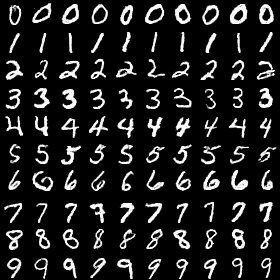
\includegraphics[width=0.48\linewidth]{figures/mnist_samples.png}}
	\subfigure[Real images~(nearest neighbor)]{
		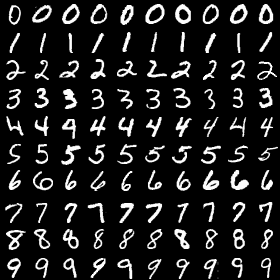
\includegraphics[width=0.48\linewidth]{figures/mnist_nn.png}}
	\subfigure[SGAN samples~(conditioned on generated \texttt{fc3} features)]{
		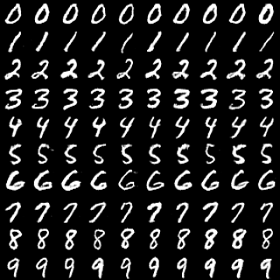
\includegraphics[width=0.48\linewidth]{figures/mnist_fc3.png}}
    \subfigure[SGAN samples~(conditioned on generated \texttt{fc3} features, trained \emph{without} entropy loss)]{
		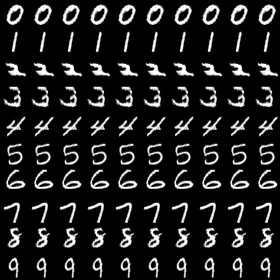
\includegraphics[width=0.48\linewidth]{figures/mnist_fc3_noent.png}}
	\caption{{\bf MNIST results.} 
(a) Samples generated by SGAN when conditioned on class labels. (b) Corresponding nearest neighbor images in the training set. (c) Samples generated by the bottom GAN when conditioned on a fixed \texttt{fc3} feature activation, generated by the top GAN. (d) Same as (c), but the bottom GAN is trained without entropy loss.} 
	\label{fig:mnist}
	\vspace{-0.2cm}
\end{figure}



\begin{figure}[!htbp]
	\centering
% 	\hspace{-0.3cm}
	\subfigure[SGAN samples~(conditioned on labels)]{
 		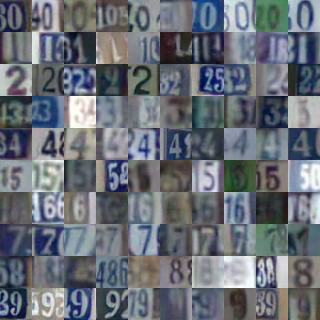
\includegraphics[width=0.48\linewidth]{figures/svhn_samples.png}}
	\subfigure[Real images~(nearest neighbor)]{
		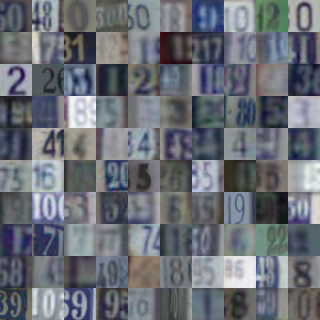
\includegraphics[width=0.48\linewidth]{figures/svhn_nn.png}}
 	\subfigure[SGAN samples~(conditioned on generated $\texttt{fc3}$ features)]{
 		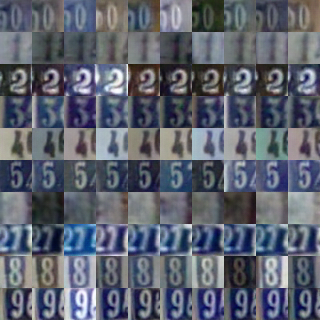
\includegraphics[width=0.48\linewidth]{figures/svhn_fc3.png}}
    \subfigure[SGAN samples~(conditioned on generated $\texttt{fc3}$ features, trained \emph{without} entropy loss)]{
		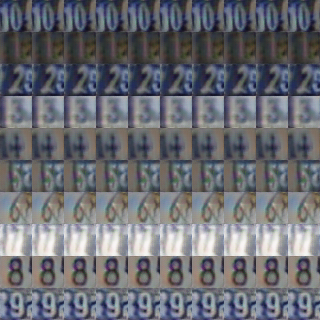
\includegraphics[width=0.48\linewidth]{figures/svhn_conditioned_fc3_noentropyloss.png}}
	\caption{{\bf SVHN results.} 
(a) Samples generated by SGAN when conditioned on class labels. (b) Corresponding nearest neighbor images in the training set. (c) Samples generated by the bottom GAN when conditioned on a fixed \texttt{fc3} feature activation, generated by the top GAN. (d) Same as (c), but the bottom GAN is trained without entropy loss.} 
 	\label{fig:svhn}
 	 \vspace{-0.2cm}
   %\vspace{-0.5em}
 \end{figure}
 
 \begin{figure}[!htbp]
	\centering
% 	\hspace{-0.3cm}
 	\subfigure[SGAN samples~(conditioned on labels)]{
 		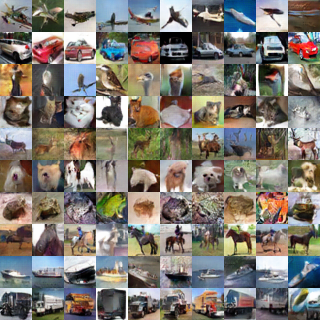
\includegraphics[width=0.48\linewidth]{figures/cifar_samples.png}}
	\subfigure[Real images~(nearest neighbor)]{
 		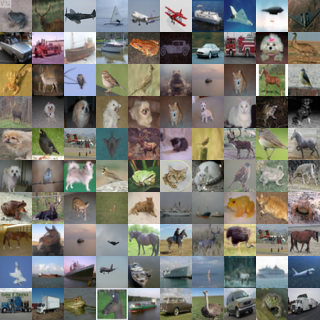
\includegraphics[width=0.48\linewidth]{figures/cifar_nn_corrected.png}}
 	\subfigure[SGAN samples~(conditioned on generated $\texttt{fc3}$ features)]{
 		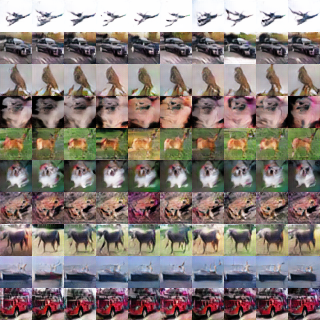
\includegraphics[width=0.48\linewidth]{figures/cifar_conditioned_fc3.png}}
    \subfigure [SGAN samples~(conditioned on generated $\texttt{fc3}$ features, trained \emph{without} entropy loss)]{
		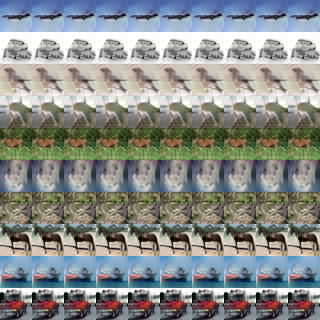
\includegraphics[width=0.48\linewidth]{figures/cifar_conditioned_fc3_noentropyloss.png}}
	\caption{{\bf MNIST results.} 
(a) Samples generated by SGAN when conditioned on class labels. (b) Corresponding nearest neighbor images in the training set. (c) Samples generated by the bottom GAN when conditioned on a fixed \texttt{fc3} feature activation, generated by the top GAN. (d) Same as (c), but the bottom GAN is trained without entropy loss.} 
 	\label{fig:cifar}
 	 \vspace{-0.2cm}
 \end{figure}
 
\subsection{Samples}
\label{samples}

In Fig.~\ref{fig:mnist}~(a), we show MNIST samples generated by SGAN. Each row corresponds to samples conditioned on a given digit class label. SGAN is able to generate diverse images with different characteristics. The samples are visually indistinguishable from real MNIST images shown in Fig.~\ref{fig:mnist}~(b), but still have differences compared with corresponding nearest neighbor training images. 

We further examine the effect of entropy loss. In Fig.~\ref{fig:mnist} (c) we show the samples generated by bottom GAN when conditioned on a fixed \texttt{fc3} feature generated by the top GAN. %, which is generated by the top GAN in the first place. 
The samples (per row) have sufficient low-level variations, which reassures that bottom GAN learns to generate images without ignoring the noise $z_0$. 
%This indicates that each GAN has the potential to capture the full conditional distribution $p(\hat{h}_{i}|h_{i+1})$.
%In other words, SGAN is capable of generating visually realistic images containing sufficient low-level details, yet without losing diversity across generated samples.  
In contrast, in Fig.~\ref{fig:mnist}~(d), we show samples generated without using entropy loss for bottom generator, where we observe that the bottom GAN ignores the noise and instead deterministically generates images from \texttt{fc3} features. 

An advantage of SGAN compared with a vanilla GAN is its interpretability: it decomposes the total variations of an image into different levels. For example, in MNIST it decomposes the variations into $y$ that represents the high-level digit label, $z_{1}$ that captures the mid-level coarse pose of the digit and $z_{0}$ that represents the low-level spatial details. %Similar decomposition can be observed in experiments on other datasets.

The samples generated on SVHN and CIFAR-10 datasets can be seen in Fig.~\ref{fig:svhn} and Fig.~\ref{fig:cifar}, respectively. Provided with the same $\texttt{fc3}$ feature, we see in each row of panel (c) that SGAN is able to generate samples with similar coarse outline but different lighting conditions and background clutters. Also, the nearest neighbor images in the training set indicate that SGAN is not simply memorizing training data, but can truly generate novel images. %This is expected because $\texttt{fc3}$ features are learned to ignore those information irrelevant to classification. Therefore, the noise variables of the bottom generator have to resolve these low-level uncertainties.

\subsection{Comparison with the state of the art}
Here, we compare SGAN with other state-of-the-art generative models on CIFAR-10 dataset. The visual quality of generated images is measured by the widely used metric, Inception score~\cite{salimans2016improved}. Following~\cite{salimans2016improved}, we sample $50, 000$ images from our model and use the code provided by~\cite{salimans2016improved} to compute the score. As shown in Tab.~\ref{tab:inception}, SGAN obtains a score of $8.59\pm 0.12$, outperforming AC-GAN~\cite{odena2017conditional} ($8.25\pm 0.07$) and Improved GAN~\cite{salimans2016improved} ($8.09\pm 0.07$). Also, note that the $5$ techniques introduced in~\cite{salimans2016improved} are not used in our implementations. Incorporating these techniques might further boost the performance of our model.

\begin{table}[!tbp]
\centering
\begin{threeparttable}
\renewcommand{\arraystretch}{1.2}
\begin{tabular}{lllll}
\hline
Method          		& Score \\ \hline
Infusion training~\cite{bordes2017learning} & $4.62\pm 0.06$ \\ 
ALI~\cite{dumoulin2017adversarially} (as reported in~\cite{david2017improving}) 				& $5.34\pm 0.05$ \\ 
GMAN~\cite{durugkar2017gman} (best variant)	& $6.00\pm 0.19$ \\ 
% LAPGAN~\cite{denton2015deep}\tnote{\ddag} & $?$ \\
EGAN-Ent-VI~\cite{dai2017calibrating} 					& $7.07\pm 0.10$ \\
LR-GAN~\cite{yang2017lrgan}	& $7.17\pm 0.07$ \\ 
Denoising feature matching~\cite{david2017improving} 					& $7.72\pm 0.13$ \\ \hline
$\text{DCGAN}^{\dag}$ (with labels, as reported in ~\cite{wang2017learning}) 		& $6.58$ \\ 
$\text{SteinGAN}^{\dag}$~\cite{wang2017learning} 		& $6.35$ \\ 
% $\text{CC-LAPGAN}^{\dag \ddag}$~\cite{denton2015deep} & $?$ \\
$\text{Improved GAN}^{\dag}$~\cite{salimans2016improved} (best variant)	& $8.09\pm 0.07$ \\ 
$\text{AC-GAN}^{\dag}$~\cite{odena2017conditional}			& $8.25\pm 0.07$ \\ \hline
DCGAN~$(\mathcal{L}^{adv})$	& $6.16\pm 0.07$ \\ 
DCGAN~$(\mathcal{L}^{adv}+\mathcal{L}^{ent})$	& $5.40\pm 0.16$ \\ 
DCGAN~$(\mathcal{L}^{adv}+\mathcal{L}^{cond})^{\dag}$	& $5.40\pm 0.08$ \\ 
DCGAN~$(\mathcal{L}^{adv}+L^{cond}+\mathcal{L}^{ent})^{\dag}$			& $7.16\pm 0.10$ \\ 
$\textbf{SGAN-no-joint}^{\dag}$	& $\textbf{8.37} \pm 0.08$ \\
$\textbf{SGAN}^{\dag}$		& $\textbf{8.59} \pm 0.12$ \\ \hline
Real data 				& $11.24\pm 0.12$ \\ 
\end{tabular}
\begin{tablenotes}
\item [\dag] Trained with labels.
% \item [\ddag] We compute the Inception score from the code provided by the authors.
\end{tablenotes}
\caption{\textbf{Inception Score on CIFAR-10.} SGAN and SGAN-no-joint outperform previous state-of-the-art approaches.}\label{tab:inception}
\end{threeparttable}
\vspace{-0.2cm}
\end{table}


\subsection{Visual Turing test}
To further verify the effectiveness of SGAN, we conduct human visual Turing test in which we ask AMT workers to distinguish between real images and images generated by our networks. We exactly follow the interface used in Improved GAN~\cite{salimans2016improved}, in which the workers are given $9$ images at each time and can receive feedback about whether their answers are correct. With $9,000$ votes for each evaluated model, our AMT workers got $24.4\%$ error rate for samples from SGAN and $15.6\%$ for samples from DCGAN~$(\mathcal{L}^{adv}+L^{cond}+\mathcal{L}^{ent})$. This further confirms that our stacked design can significantly improve the image quality over GAN without stacking.

% We also show qualitative comparisons between SGAN and Improved GAN~\cite{salimans2016improved}, the published state-of-the-art model on CIFAR-10 dataset (we do not have access to either the CIFAR-10 samples or code of AC-GAN~\cite{odena2017conditional} at the time of writing). 

\subsection{More ablation studies}
In Sec.~\ref{samples} we have examined the effect of entropy loss. In order to further understand the effect of different model components, we conduct extensive ablation studies by evaluating several baseline methods on CIFAR-10 dataset. If not mentioned otherwise, all models below use the same training hyper-parameters as the full SGAN model.
\begin{enumerate}[(a)]
\item SGAN: The full model, as described in Sec.~\ref{methods}.
\item SGAN-no-joint: Same architecture as (a), but each GAN is trained \emph{independently}, and there is no final joint training stage. %This is similar to LAPGAN~\cite{denton2015deep} where GANs at each resolution are trained independently.
\item DCGAN~($\mathcal{L}^{adv}+\mathcal{L}^{cond}+\mathcal{L}^{ent}$): This is a \emph{single} GAN model with the same architecture as the bottom GAN in SGAN, except that the generator is conditioned on labels instead of \texttt{fc3} features. Note that other techniques proposed in this paper, including conditional loss $\mathcal{L}^{cond}$ and entropy loss $\mathcal{L}^{ent}$, are still employed. We also tried to use the full generator $G$ in SGAN as the baseline, instead of only the bottom generator $G_{0}$. However, we failed to make it converge, possibly because $G$ is too deep to be trained without intermediate supervision from representation discriminators.
\item DCGAN~($\mathcal{L}^{adv}+\mathcal{L}^{cond}$): Same architecture as (c), but trained without entropy loss $\mathcal{L}^{ent}$.
\item DCGAN~($\mathcal{L}^{adv}+\mathcal{L}^{ent}$): Same architecture as (c), but trained without conditional loss $\mathcal{L}^{cond}$. This model therefore does not use label information.
\item DCGAN~($\mathcal{L}^{adv}$): Same architecture as (c), but trained with neither conditional loss $\mathcal{L}^{cond}$ nor entropy loss $\mathcal{L}^{ent}$. This model also does not use label information. It can be viewed as a plain unconditional DCGAN model~\cite{radford2016unsupervised} and serves as the ultimate baseline.
\end{enumerate}


 \begin{figure}[!tbp]
	\centering
 		\subfigure[SGAN]{
 		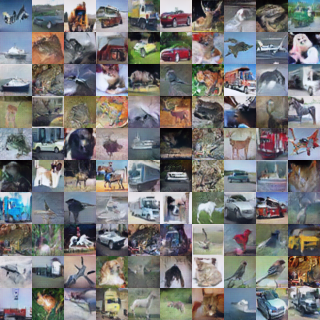
\includegraphics[width=0.48\linewidth]{figures/cifar_random.png}}        
 		\subfigure[SGAN-no-joint]{
 		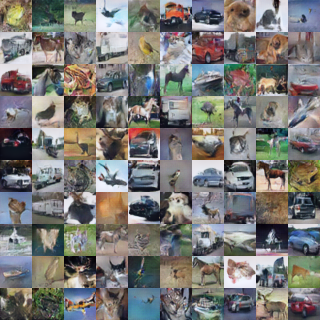
\includegraphics[width=0.48\linewidth]{figures/cifar_nojoint_random.png}}        
    	\subfigure [\hspace{-0.06cm}DCGAN\hspace{0.03cm}($\mathcal{L}^{adv}+\mathcal{L}^{cond}+\mathcal{L}^{ent})$]{
		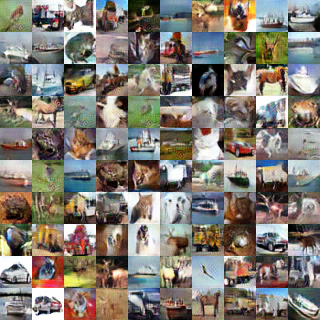
\includegraphics[width=0.48\linewidth]
        {figures/cifar_nojoint_nostack_random.png}}        
    	\subfigure [DCGAN~($\mathcal{L}^{adv}+\mathcal{L}^{cond}$)]{
		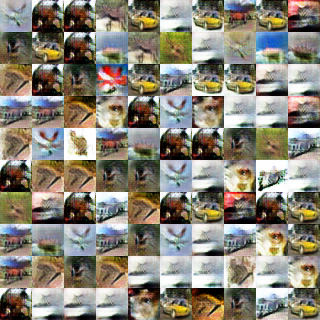
\includegraphics[width=0.48\linewidth]
        {figures/cifar_nojoint_nostacknoent_random.png}}        
    	\subfigure [DCGAN~($\mathcal{L}^{adv}+\mathcal{L}^{ent}$)]{
		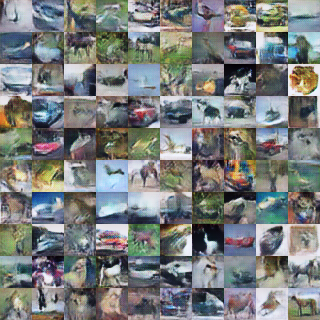
\includegraphics[width=0.48\linewidth]
        {figures/cifar_nojoint_nostacknofea_random.png}}        
        \subfigure [DCGAN~($\mathcal{L}^{adv}$)]{
		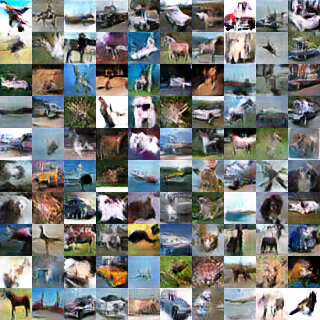
\includegraphics[width=0.48\linewidth]
        {figures/cifar_nojoint_nostacknoentnofea_random.png}}
 	\caption{{\bf Ablation studies on CIFAR-10.} Samples from (a) full SGAN (b) SGAN without joint training. (c) DCGAN trained with $\mathcal{L}^{adv}+\mathcal{L}^{cond}+\mathcal{L}^{ent}$ (d) DCGAN trained with $\mathcal{L}^{adv}+\mathcal{L}^{cond}$ (e) DCGAN trained with $\mathcal{L}^{adv}+\mathcal{L}^{ent}$ (f) DCGAN trained with $\mathcal{L}^{adv}$. } 
 	\label{fig:ablation}
 	 \vspace{-0.2cm}
 \end{figure}

We compare the generated samples~(Fig.~\ref{fig:ablation}) and Inception scores~(Tab.~\ref{tab:inception}) of the baseline methods. Below we summarize some of our results:
\begin{enumerate}[1)]
\item SGAN obtains slightly higher Inception score than SGAN-no-joint. %This is not surprising, because error of the top GAN may accumulate to the bottom GAN without joint training. 
Yet SGAN-no-joint also generates very high quality samples and outperforms all previous methods in terms of Inception scores. 
%We also observe that joint training is more apt to (partial) model collapse and additional caution needs to be taken, such as adding Gaussian noise to the discriminators.
\item SGAN, either with or without joint training, achieves significantly higher Inception score and better sample quality than the baseline DCGANs. This demonstrates the effectiveness of the proposed stacked approach.
\item As shown in Fig.~\ref{fig:ablation}~(d), DCGAN~($\mathcal{L}^{adv}+\mathcal{L}^{cond}$) collapses to generating a single image per category, while adding the entropy loss enables it to generate diverse images (Fig.~\ref{fig:ablation}~(c)). This further demonstrates that entropy loss is effective at improving output diversity.
%\item The plain unconditional DCGAN~($\mathcal{L}^{adv}$) does not collapse and obtains competitive Inception score compared with some previous models. In this case, adding entropy loss $\mathcal{L}^{ent}$ does not seem to provide benefits, at least in terms of the Inception score (Tab.~\ref{tab:inception}).
\item The single DCGAN ($\mathcal{L}^{adv}+\mathcal{L}^{cond}+\mathcal{L}^{ent}$) model obtains higher Inception score than the conditional DCGAN reported in~\cite{wang2017learning}. This suggests that $\mathcal{L}^{cond}+\mathcal{L}^{ent}$ might offer some advantages compared to a plain conditional DCGAN, even without stacking.
\item In general, Inception score~\cite{salimans2016improved} correlates well with visual quality of images. However, it seems to be insensitive to diversity issues							. For example, it gives the same score to Fig.~\ref{fig:ablation}~(d) and (e) while (d) has clearly collapsed. This is consistent with results in~\cite{odena2017conditional,wang2017learning}.
\end{enumerate}





% \subsection{MNIST}
% %We use a SGAN architecture with only two stacks, since MNIST dataset has relatively small variations across images. 
%  %In practice, we find using mini-batch discrimination \cite{salimans2016improved} alone is sufficient to impose diversity for the top GAN, while entropy loss is necessary for training the bottom GAN.
% The MNIST dataset contains $60,000$ labeled images of digits.  In Figure~\ref{fig:mnist} (b), we show MNIST samples generated by SGAN when feeding both $z_0$ and $z_1$ with random noise. The samples are visually indistinguishable from real MNIST images shown in Figure~\ref{fig:mnist} (a). When conditioned on a given label, SGAN is able to generate diverse images with inherently different characteristics (see Figure~\ref{fig:mnist} (d)). 

% We further examine the effect of entropy loss (Section~\ref{Entloss}). We show in Figure~\ref{fig:mnist} (e) samples generated by bottom GAN when conditioned on a fixed \texttt{fc3} feature, which is generated by the top GAN in the first place. The samples (per row) have sufficient low-level variations. And this reassures that bottom GAN learns to generate images without ignoring the noise $z_0$. In other words, SGAN is capable of generating visually realistic images containing sufficient low-level details, yet without losing diversity across generated samples.  In contrast, in Figure~\ref{fig:mnist} (f), we show samples generated without using entropy loss, where we observe the lack of diversity across generated samples since the bottom GAN ignores the noise and instead deterministically generates images from \texttt{fc3} features. 

% An advantage of SGAN compared with a vanilla GAN is its interpretability: it decomposes total variations of an image into different levels. For example, in MNIST it decomposes the variations into $y$ that represents the high-level digit label, $z_{1}$ that captures the mid-level coarse pose of the digit, $z_{0}$ that represents the low-level spatial details. Similar decomposition can be observed in experiments on other datasets.

%We first show some random generated results (randomly sampling everything).
% \begin{figure*}[!htbp]
% \centering
% \includegraphics[width=0.8\linewidth]{figures/mnist_random.png}
%    \caption{Random generation on MNIST. }
% \label{fig:mnist}
% \end{figure*}



% \begin{figure*}[h]
% 	\centering
% 	\hspace{-0.3cm}
% 	\subfigure[Real images]{
% 		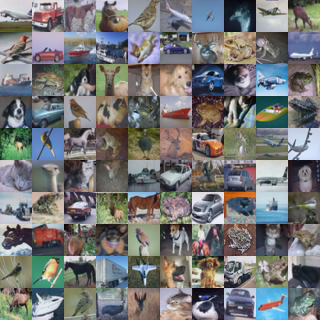
\includegraphics[width=0.25\linewidth]{figures/cifar_real.png}}
%      \subfigure[SGAN samples]{
% 		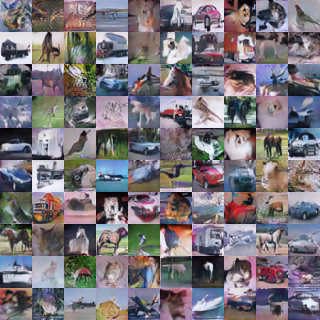
\includegraphics[width=0.25\linewidth]{figures/cifar_sgan_epoch220.png}}
%      \subfigure[Baseline samples]{
% 		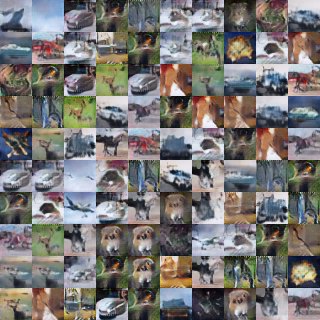
\includegraphics[width=0.25\linewidth]{figures/cifar_base.png}}
% 	\caption{{\bf CIFAR results.} (a) Real CIFAR images. (b) Samples generated by SGAN when feeding both stacks with random noise. (c) Samples generated by the baseline method. The diversity and quality of baseline samples are significantly worse than samples from SGAN.} 
% 	\label{fig:cifar}
% \end{figure*}



% \subsection{SVHN}
% We further evaluate our model on the Street View House Numbers (SVHN) dataset, a digit classification benchmark which is composed of real-world color images of house numbers collected by Google Street View \cite{netzer2011reading}. Each image is of size $32\times32$ and the task is to classify the digit at the center of the image. %Nearby digits and other distractors are kept in the image, which makes the classification task more challenging. 
% The dataset contains $73,257$ images in the training set and $26,032$ images in the test set. 

% The results are shown in Figure~\ref{fig:svhn}. Most of the the generated SGAN samples in figure~\ref{fig:svhn} (b) are visually indistinguishable from the real SVHN images in figure~\ref{fig:svhn} (a). Here the baseline model suffers from the missing mode problem (see Figure~\ref{fig:svhn} (c)), concentrating its probability mass around a few data points. Our SGAN is able to generate much more diverse images (see Figure~\ref{fig:svhn} (b)), partially due to the use of entropy loss. Provided with the same $\texttt{fc3}$ feature, we see in each row of Figure~\ref{fig:svhn} (e) that SGAN is able to generate samples with similar coarse outline but different lighting conditions and background clutters. This is expected because $\texttt{fc3}$ features are learned to ignore those information irrelevant to classification. Therefore, the noise variables of the bottom generator have to resolve these low-level uncertainties. Furthermore, the effect of using entropy loss can be observed from comparing Figure~\ref{fig:svhn} (e) and (f).

%We use a SGAN architecture with two stacks. The top GAN generates \texttt{fc3} features from random noise, conditioned on label information. The bottom GAN generates images from random noise, conditioned on \texttt{fc3} features generated by the top GAN. Results are shown in figure~\ref{fig:svhn}. As shown in the supplementary material, the diversity and quality of samples from SGAN are superior to those generated by the baseline method. Moreover, without using entropy loss, the generated images of the bottom GAN given the same $\texttt{fc3}$ feature lack diversity.%Using the VGG-like encoder described in the previous subsection, we achieved $95.5\%$ accuracy on the validation set. 

% \begin{figure}[h]
% 	\centering
% 	\hspace{-0.3cm}
% 	\subfigure[Real images]{
% 		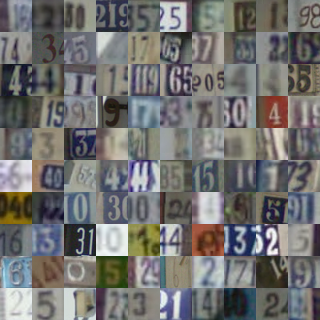
\includegraphics[width=0.49\linewidth]{figures/svhn_real.png}}
%      \subfigure[SGAN samples]{
% 		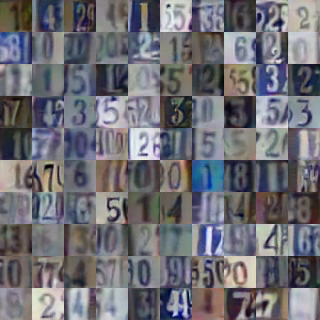
\includegraphics[width=0.49\linewidth]{figures/svhn_sgan.png}}
% 	\caption{{\bf SVHN results.} (a) Real SVHN images. (b) Samples generated by SGAN when feeding both stacks with random noise. Zoom in for details. } 
% 	\label{fig:svhn}
% \end{figure}

% \subsection{CIFAR}


% % \begin{figure}[h]
% % 	\centering
% % 	\hspace{-0.3cm}
% % 	\subfigure[Real images]{
% % 		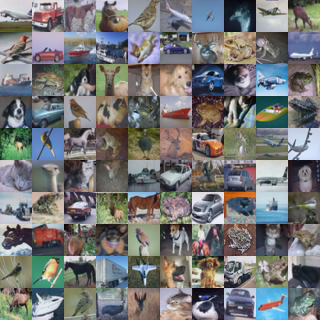
\includegraphics[width=0.49\linewidth]{figures/cifar_real.png}}
% %      \subfigure[SGAN samples]{
% % 		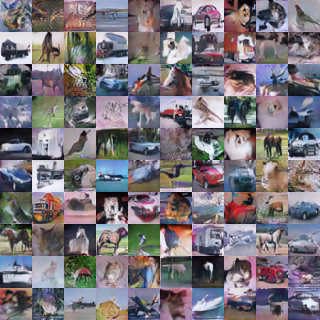
\includegraphics[width=0.49\linewidth]{figures/cifar_sgan_epoch220.png}}
% % 	\caption{{\bf CIFAR results.} (a) Real CIFAR images. (b) Samples generated by SGAN when feeding both stacks with random noise. Zoom in for details. } 
% % 	\label{fig:cifar}
% % \end{figure}

% The CIFAR-10 dataset consists of colored natural scene images sized at $32\times 32$ pixels. There are 50,000 training images and 10,000 test images in $10$ classes. The results are shown in Figure~\ref{fig:cifar}. To quantitatively measure the image quality, we compute the widely used metric, Inception score~\cite{salimans2016improved}. Our SGAN approach obtains Inception score of $7.22\pm 0.11$, higher than the baseline model ($5.79\pm 0.15$). Similar to the results on SVHN, the baseline model also suffers from the missing mode problem (see Figure~\ref{fig:cifar} (c)).   %, which is consistent with our visual inspection.


\section{Discussion and Future Work}
\label{discussion}

This paper introduces a top-down generative framework named SGAN, which effectively leverages the representational information from a pre-trained discriminative network. Our approach decomposes the hard problem of estimating image distribution into multiple relatively easier tasks -- each generating plausible representations conditioned on higher-level representations. The key idea is to use representation discriminators at different training hierarchies to provide intermediate supervision. We also propose a novel entropy loss to tackle the problem that conditional GANs tend to ignore the noise. Our entropy loss could be employed in other applications of conditional GANs, \emph{e.g.}, synthesizing \emph{different} future frames given the same past frames~\cite{mathieu2016deep}, or generating a \emph{diverse} set of images conditioned on the same label map~\cite{pix2pix2016}. We believe this is an interesting research direction in the future.

%Our  approach raises several interesting future directions to explore: (1) semi-supervised or unsupervised training of hierarchical generative models. This can be fruitful for many situations when the labeled examples are insufficient.  (2) a more principled way for grouping ``stacks'' of generators during hierarchical training, such that the total entropy of image can be evenly distributed across all stacks. (3) visualizing and understanding the intermediate features in deep networks with SGAN.

%Our method is motivated by the fact that current bottom-up discriminative networks are far more powerful than top-down generative networks. With adversarial training, we transfer the knowledge in bottom-up networks to the top-down networks. H
%However, there are situations when training powerful bottom-up networks is also difficult due to limited number of labels available. In the future we plan to train the top-down generative model and the bottom-up discriminative model jointly in an unsupervised or semi-supervised way, and study whether our  generative \& discriminative feature learning could simultaneously help each other. Moreover, the formation of "stack" is currently arbitrary. We plan to investigate an automatic way of defining "stack" such that the total entropy of the image is approximately evenly distributed across all stacks, \emph{i.e.}, $H(h_{i}|h_{i+1})=\frac{H(x)-H(y)}{N}$ for all $i$, in order to make the task difficulty more balanced across each GAN. 

\subsubsection*{Acknowledgments}

We would like to thank Danlu Chen for the help with Fig.~\ref{fig:sgan}. Also, we want to thank Danlu Chen, Shuai Tang, Saining Xie, Zhuowen Tu, Felix Wu and Kilian  Weinberger for helpful discussions.  Yixuan Li is supported by US Army Research Office W911NF-14-1-0477. Serge Belongie is supported in part by a Google Focused Research Award.

{\small
\bibliographystyle{ieee}
\bibliography{egbib}
}

\end{document}
